%!TEX root = ../thesis.tex

% https://en.wikipedia.org/wiki/Kelly_Johnson_(engineer)
% https://en.wikipedia.org/wiki/KISS_principle
\begin{savequote}[40mm]
	\textbf{K}eep\\
	\textbf{I}t\\
	\textbf{S}imple\\
	\textbf{S}tupid
	\qauthor{Kelly Johnson}
\end{savequote}

\chapter{Proposed solution}\label{chapter:proposed_solution}
	
	% TODO AGGIUNGERE UNA O DUE FRASI?

	This chapter contains the technical description of the mesh network developed with the FiPy and communicates using LoRa.
	Especially such networks is able to accommodate small messages, such as the ones sent by MegaSense, described in Section \ref{subsec:megasense}.
		
	Even though it would have been possible to use a simulator, such as ``The one'' \footnote{ \url{http://akeranen.github.io/the-one/}}, for demonstrating the usefulness of such network, the final project has been realized with Pycom hardware.
	
	\section{Architecture}\label{sec:architecture}
		
		Before talking about the architecture of the mesh, it is important to understand the one of the MegaSense.
		As can be seen in Figure~\ref{img:megasense_architecture}, since each MegaSense device is made to be carried by a person, devices connect each one to the user's phone.
		The latter then communicates with the MegaSense and, via the application developed by the Computer Science department at the University of Helsinki, sends the air-quality readings and the GPS location, which has been read by the application from the phone itself, to the servers in the cloud.
		
		Communication between MegaSense and phone is done via BLE, and exchanges data such as battery status, 
		
		\begin{figure}
			\centering
			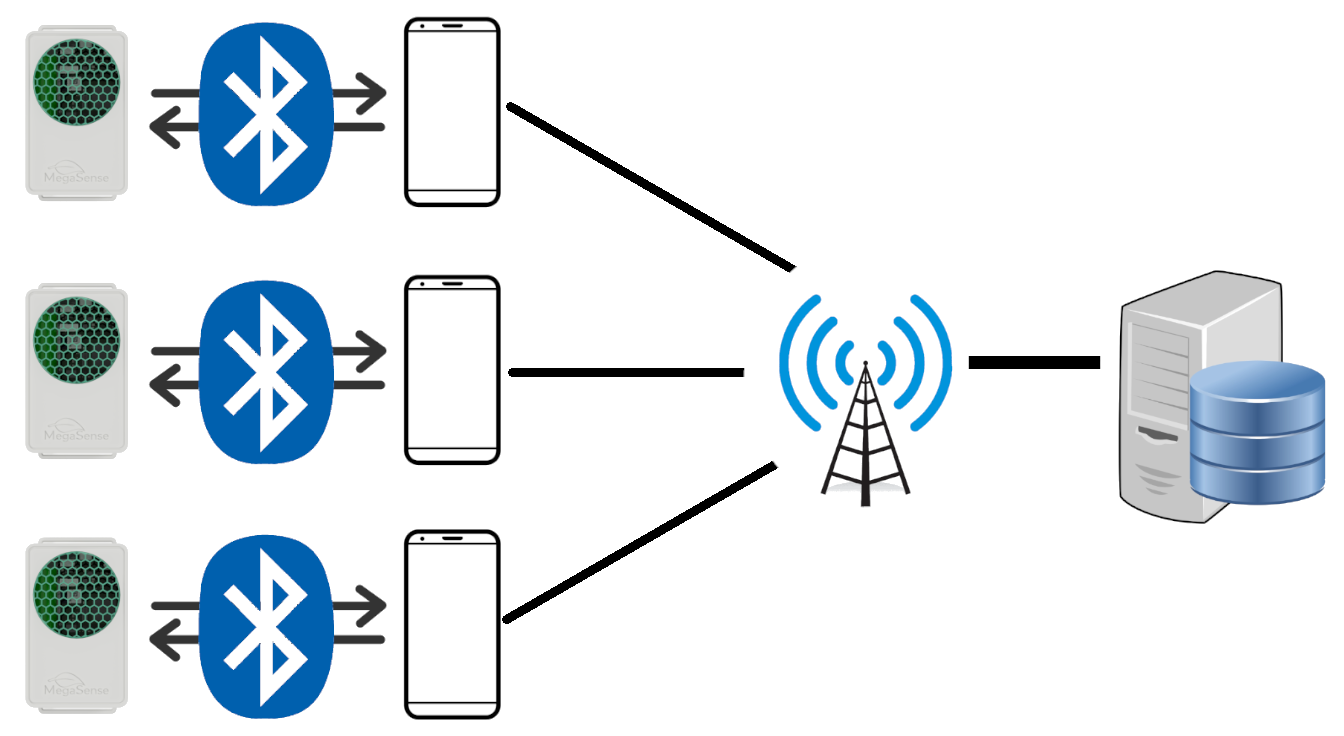
\includegraphics[width=.8\textwidth]{resources/img/chap5/architecture_megasense}
			\caption{MegaSense architecture}
			\label{img:megasense_architecture}
		\end{figure}
	
		
		
		
		
		Each FiPy board represents a node on the network, which in this case is a ``Flat Wireless Mesh''.
	
		Flat Wireless Mesh
		
		Typically, in a wired or wireless network, clients are data providers and routers
		are used as data forwarders. But, in a flat WMN, all the nodes are seen as peers. \cite{92000412}
	
		% TODO inserire immagine per architettura
		
		As represented in Figure \ref{img:mesh_architecture}, the network is composed of 
	
	\section{Hardware}
	
		%Describe hardware requirements, connect to the sections in chap 3 
		%
		%Altri microcontroller, come esp8266 che sono stati generati da arduino sono stati scartati in quanto poca documentazione, ecc
	
	\section{Software}
	
	% Hardware Addressing Schemes
	
	
	% https://www.circuitbasics.com/basics-uart-communication/
	%UART
	%
	%How I programmed the pycom
	
	% Author's note, I believe that, due to some lack of documentation from the board manufacturer's webpage, I believe it is important to include in this thesis some technical points on how the boards have been programmed (oppure meglio mettere in un'appendice a parte??? Forse meglio perchè in questo caso si vanno a separare i concetti che riguardano direttamente la tesi da quelli che riguardano )
	%
	%
	%calcolare transmission times
	
		While the Arduino C++ divides the code in two main functions, the \texttt{setup()} and \texttt{loop()}, as mentioned in Chap. \ref{chapter:technologies}, the Pycom boards use two files to separate an initial bootstrap of the board and a main section of the code.
		These two special files are called \texttt{boot.py} and \texttt{main.py} respectively.
		
		The next section explains the algorithms made for this project and how they are implemented.
		
		\subsection{Algorithms}\label{subsec:algorithms}
	
			% https://latexdraw.com/automata-diagrams-in-latex/
			% https://hayesall.com/blog/latex-automata/
			% https://isaaccomputerscience.org/concepts/dsa_toc_fsm?examBoard=all&stage=all
		
			Finite-state machine
		
			To better understand the algorithms, they are represented using finite state machines.
			For a graphical reason, each state of the automatas is abbreviated, and the full state is described in a table underneath
			
			Visione da generale a specifica di ciasun componente
			
			As said previously, the code is divided in two files, boot.py
			
			\subsubsection{Main}
				
				\begin{center}
	
					\begin{tikzpicture}[shorten >=1pt,node distance=2cm,on grid,auto]
					
						% Help grid
						% \draw [help lines] (-1,1) grid (6,-6);
						
						\tikzstyle{every state}=[fill={rgb:black,1;white,10}]
						
	
						\node[state, initial]  			(s_0)                 	{$s_0$}; % START
						\node[state] 					(s_1)	[right of=s_0]	{$s_1$}; % BOOT
						\node[state]					(s_2) 	[right of=s_1]	{$s_2$}; % MESH DEFINITION
						\node[state, accepting]			(s_3) 	[right of=s_2]	{$s_3$}; % MAIN LOOP
						
						\path[->]
						(s_0) edge node {} (s_1)
						(s_1) edge node {} (s_2)
						(s_2) edge node {} (s_3)
						(s_3) edge [loop right] node {} ();
					
					\end{tikzpicture}
					
				\end{center}

				\begin{table}[htbp]
					\begin{center}
						\begin{tabularx}{0.85\textwidth}{@{}|Y|Y|Y|@{}} 
							\hline
							State abbreviation & Full state name & State description \\\hline
							$s_{0}$ && \\\hline
						\end{tabularx}
						\caption{Main algorithm fsm description}
						\label{table:fsm_main}
					\end{center}
				\end{table}
							
				\begin{center}
					
					% BLOCK STYLES
					\tikzstyle{decision} = [diamond, draw, fill=blue!20, text width=4.5em, text badly centered, node distance=3cm, inner sep=0pt]
					\tikzstyle{block} = [rectangle, draw, fill=blue!20,	text width=4em, text centered, rounded corners, minimum height=3em]
					\tikzstyle{line} = [draw, -latex']
					\tikzstyle{cloud} = [draw, ellipse,fill=red!20, minimum height=2.5em, minimum width=3.5em]

					\begin{tikzpicture}[node distance = 2cm, auto]
						
						% BLOCKS
						
						\node [cloud] 					(start) 	{start};
						\node [block, below of=start] 	(boot) 		{boot()};
						\node [block, below of=boot] 	(main) 		{main()};
						\node [cloud, below of=main] 	(end) 		{end};
						
						% EDGES
						\path [line] (start) -- (boot);
						\path [line] (boot) -- (main);
						\path [line] (main) -- (end);
						
					\end{tikzpicture}

				\end{center}
	
			\subsubsection{Boot up}
			
			\subsubsection{Mesh initiation}
			
			\subsubsection{Broadcast mesh information}
			
			\subsubsection{Loop}
			
		\subsection{Sleep cycle}
		
			% TODO giustificare il fatto che non ci siano cicli di sleep in quanto se ci fossero allora la rete mesh potrebbe subire  modifiche nel durante, se un nodo va in sleep potrebbe essere che non riesce a forwardare dei messaggi che gli arrivano
			
		\subsection{Supported messages}
				
			% TODO spiegare i messaggi che vengono mandati tra i dispositivi
		
	\section{Other files}
			
	\section{Use cases}
		
		% TODO fare disegni dei use cases
		
		\subsection{Mobile network}
		
		\subsection{Fixed network}
		
		\subsection{Hybrid network}